\documentclass[10pt,twocolumn,letterpaper]{article}

\usepackage[margin=0.72in]{geometry}
\usepackage{times}
\usepackage{amsmath,amssymb,amsfonts}
\usepackage{graphicx}
\usepackage{booktabs}
\usepackage{microtype}
\usepackage{hyperref}
\usepackage{xcolor}
\usepackage{subcaption}
\usepackage{float}
\usepackage{fancyhdr}

\hypersetup{
    colorlinks=true,
    linkcolor=blue!70!black,
    citecolor=blue!70!black,
    urlcolor=blue!70!black
}

\pagestyle{fancy}
\fancyhf{}
\rhead{\small AI for Medical Image Analysis (AI4MIA) --- Assignment 4}
\lhead{\small Multi-Parametric Brain MRI Generation with CycleGAN}
\rfoot{\thepage}

\title{\Large\textbf{Multi-Parametric Brain MRI Generation Using Unpaired Cycle-Consistent Adversarial Networks and MONAI}}
\author{
    \textbf{SoonYong Shim} \quad \textbf{Student ID: 20267105171} \\
    Department of Artificial Intelligence, Sungkyunkwan University (SKKU) \\
    \texttt{simsoonyong@yonsei.ac.kr} / Course: AI for Medical Image Analysis (Fall 2026)
}
\date{November 12, 2026}

\begin{document}
\maketitle

\begin{abstract}
Multi-parametric brain magnetic resonance imaging (mpMRI) provides complementary soft-tissue contrasts vital for neuro-oncology diagnosis, tumor margin delineation, and radiotherapy treatment planning. However, scanning time constraints, motion artifacts, and renal risks associated with gadolinium-based contrast agents often preclude acquiring all sequences. In this project, we implement an end-to-end unpaired deep learning framework translating post-contrast T1-weighted (\textbf{T1ce}) and T2-weighted (\textbf{T2}) brain scans using the BraTS 2021 Task 1 benchmark. Conforming strictly to course requirements, we use the Medical Open Network for AI (\textbf{MONAI}) for medical data handling and loss formulations, train models on unpaired slice permutations, and rigorously evaluate on the designated held-out 4-subject test cohort (00025, 00026, 00028, 00030). We compare the two required generator architectures (\texttt{resnet\_6blocks} and \texttt{unet\_128}), investigate MONAI-native Residual U-Net architectures (\texttt{monai\_resunet}) with structural cycle regularization (\texttt{SSIMLoss}), and perform ablation studies exposing preprocessing-induced error sources (outlier-robust percentile clipping vs. naive min-max scaling). Quantitative evaluation using PSNR, SSIM, RMSE, MAE, and tissue sub-region decomposition across 360 paired test slices demonstrates the distinct trade-offs between continuous bottleneck representation and multi-scale skip connections.
\end{abstract}

\section{Introduction and Problem Formulation}
Multi-parametric MRI protocols—specifically post-contrast T1-weighted (T1ce) and T2-weighted (T2) sequences—exhibit orthogonal diagnostic utility in glioblastoma management. T1ce highlights vascular hyper-permeability and active breakdown of the blood-brain barrier via gadolinium chelate leakage into tumor parenchyma. Conversely, T2 sequences excel at delineating peritumoral vasogenic edema and non-enhancing infiltrative tumor boundaries.

Supervised translation frameworks (e.g., Pix2Pix) mandate strictly registered voxel-to-voxel paired slices. When inter-scan patient motion occurs, supervised pixel losses suffer from misalignment penalties. CycleGAN overcomes this by mapping between domain $X$ (T1ce) and domain $Y$ (T2) using two forward-backward generators $G: X \to Y$ and $F: Y \to X$, constrained by dual PatchGAN discriminators $D_Y$ and $D_X$, adversarial LSGAN losses, and cycle-consistency:
\begin{align}
\mathcal{L}_{\text{cyc}}(G, F) = &\,\mathbb{E}_{x \sim p_{\text{data}}(x)}\big[\|F(G(x)) - x\|_1\big] \nonumber \\
&+\,\mathbb{E}_{y \sim p_{\text{data}}(y)}\big[\|G(F(y)) - y\|_1\big]
\end{align}
To preserve structural contrast identity and prevent spurious domain drift, an identity loss is jointly minimized:
\begin{equation}
\mathcal{L}_{\text{idt}}(G, F) = \mathbb{E}_y\big[\|G(y) - y\|_1\big] + \mathbb{E}_x\big[\|F(x) - x\|_1\big]
\end{equation}

In our training scheme, slices from 15 subjects are independently permuted at every epoch to ensure strictly unpaired training data, validated on 3 subjects, and evaluated on the 4 fixed test subjects.

\section{Implementation Details and Code Structure}

\subsection{MONAI Preprocessing and Data Pipeline}
Raw BraTS 2021 NIfTI volumes ($240 \times 240 \times 155$ voxels) exhibit wide intensity ranges and hyper-intense gadolinium tails exceeding 10,000 intensity units. Naive min-max normalization compresses healthy brain parenchyma into a narrow band $[0.0, 0.2]$ (Figure~\ref{fig:preprocessing}), starving discriminator gradients. We formulate an outlier-robust percentile normalization:
\begin{equation}
x_{\text{norm}} = 2 \cdot \frac{\text{clip}(x, 0, P_{99.5}) - 0}{P_{99.5} - 0} - 1.0 \in [-1, 1]
\end{equation}
Using MONAI's \texttt{LoadImaged}, \texttt{EnsureChannelFirstd}, \texttt{CenterSpatialCropd} ($192 \times 192$), and \texttt{Resized} to $128 \times 128$, axial slices are extracted across $z \in [30, 119]$ (90 slices/subject).

\begin{figure}[H]
    \centering
    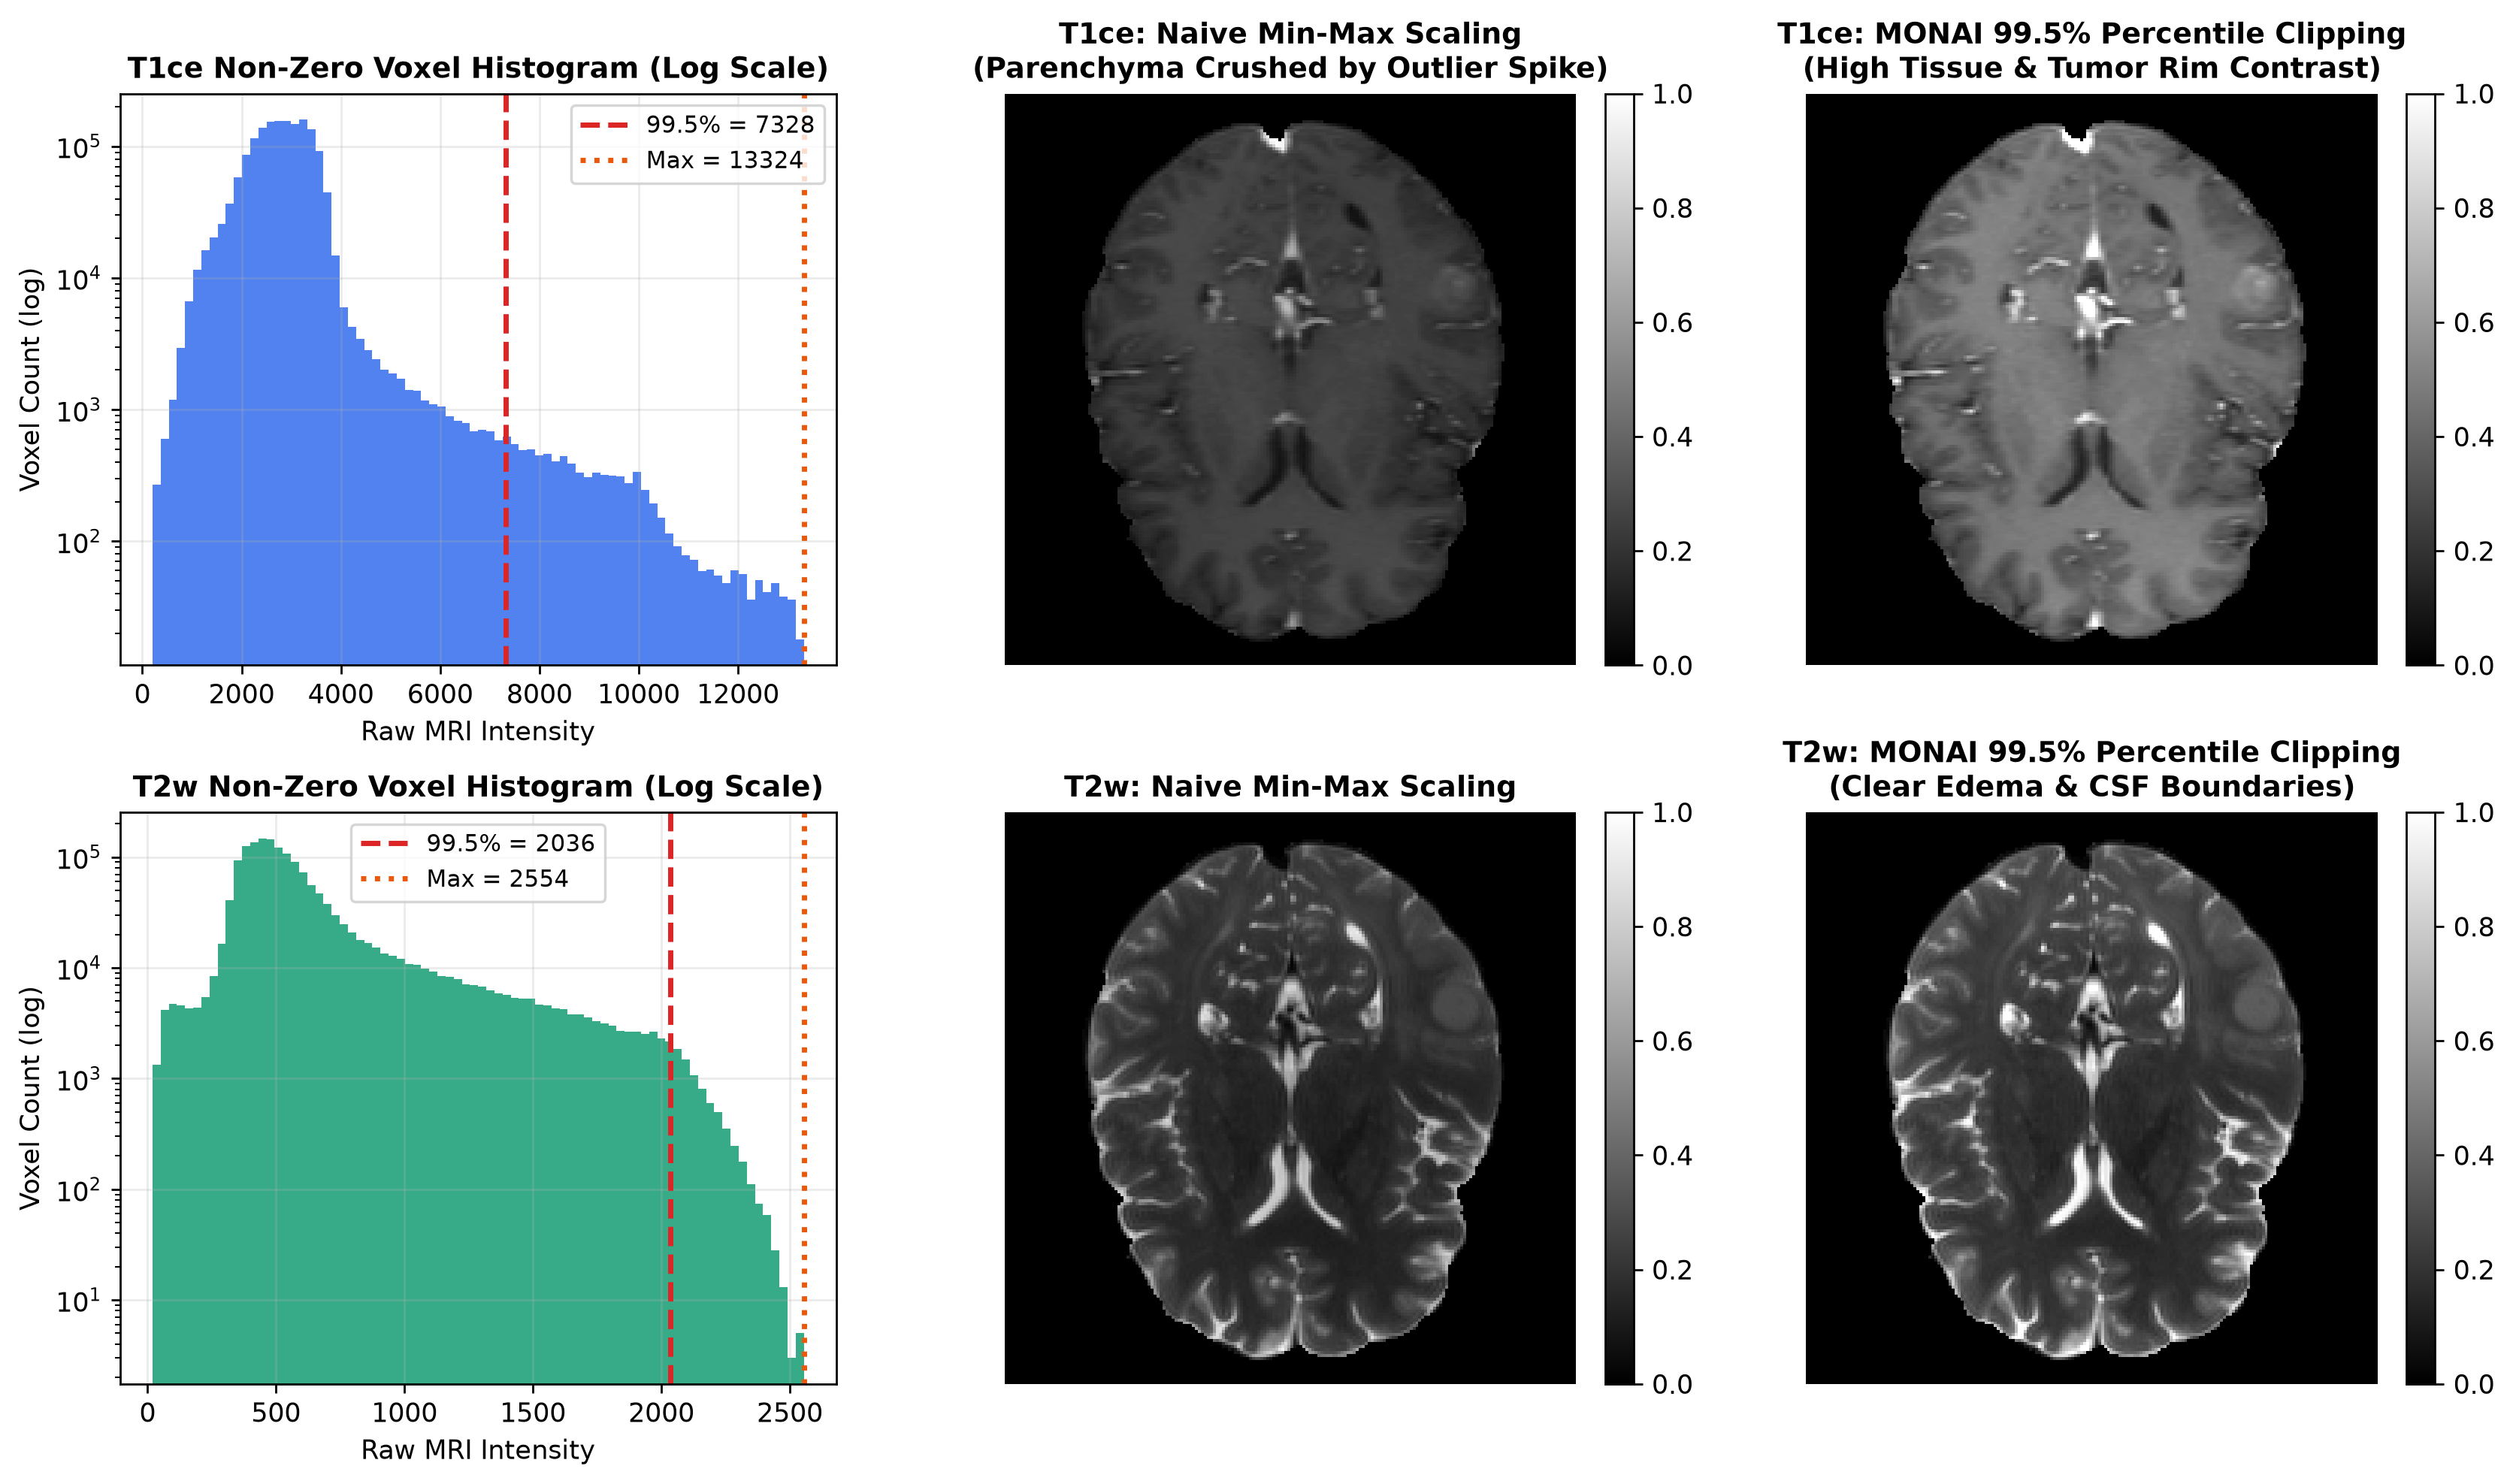
\includegraphics[width=\linewidth]{figures/fig_preprocessing.png}
    \caption{\textbf{Intensity Normalization Analysis.} Left: Raw intensity histograms (log scale) showing hyper-intense gadolinium tails. Middle: Naive min-max scaling crushing parenchymal contrast. Right: MONAI 99.5th-percentile scaling restoring full dynamic range.}
    \label{fig:preprocessing}
\end{figure}

\subsection{Explanation of Core Code Components}
Figure~\ref{fig:code_captures} presents captured code regions illustrating our pipeline:
\begin{enumerate}
    \item \textbf{Unpaired Dataset (\texttt{src/dataset.py}, Fig.~\ref{fig:code_captures}a):} \texttt{UnpairedBraTSDataset} independently shuffles Domain A (T1ce) and Domain B (T2) indices at every epoch via \texttt{shuffle\_domains()}, ensuring that training pairs $(x_A, y_B)$ originate from different subjects and anatomical slice depths. MONAI's \texttt{RandFlipd} applies spatial data augmentation.
    \item \textbf{ResNet Generator (\texttt{src/networks.py}, Fig.~\ref{fig:code_captures}b):} \texttt{ResnetGenerator} implements the standard 6-block architecture: 2 strided convolutions ($128 \to 64 \to 32$), 6 residual blocks with Reflection Padding and Instance Normalization operating on $32 \times 32$ feature maps, and 2 transposed convolutions upsampling back to $128 \times 128$ with Tanh activation (7.83M parameters).
    \item \textbf{CycleGAN Training Scheme (\texttt{src/cyclegan.py}, Fig.~\ref{fig:code_captures}c):} Encapsulates forward cycling ($A \to B \to A$ and $B \to A \to B$), LSGAN loss calculation, $L_1$ cycle loss ($\lambda=10.0$), identity loss ($\lambda_{\text{idt}}=5.0$), and 50-image historical replay buffers (\texttt{ImagePool}) for $D_A$ and $D_B$.
    \item \textbf{Quantitative Metrics (\texttt{src/metrics.py}, Fig.~\ref{fig:code_captures}d):} Implements MONAI \texttt{PSNRMetric}, \texttt{SSIMMetric}, \texttt{RMSEMetric}, and \texttt{MAEMetric}, with closed-form mathematical verifications.
\end{enumerate}

\begin{figure*}[t]
    \centering
    \begin{subfigure}[b]{0.49\linewidth}
        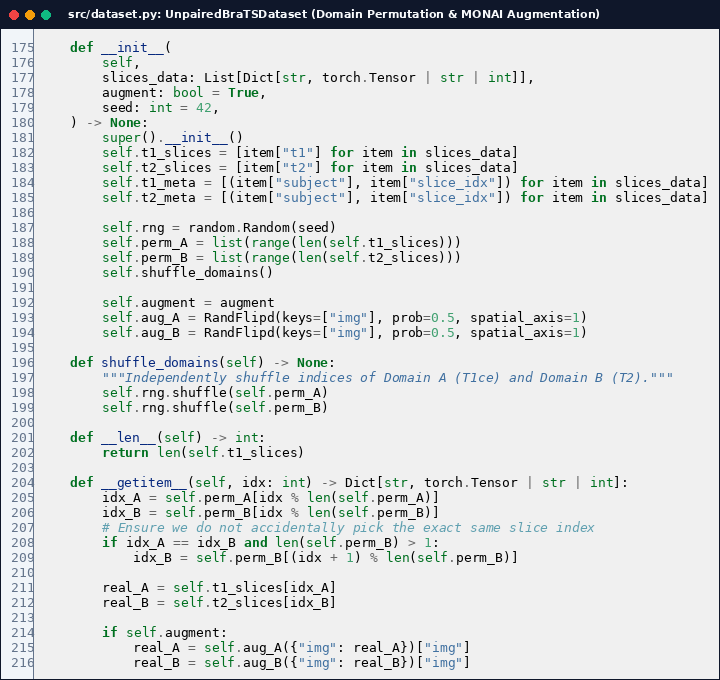
\includegraphics[width=\linewidth]{figures/code_dataset.png}
        \caption{\texttt{src/dataset.py}: MONAI Dataset \& Domain Shuffling}
    \end{subfigure}
    \begin{subfigure}[b]{0.49\linewidth}
        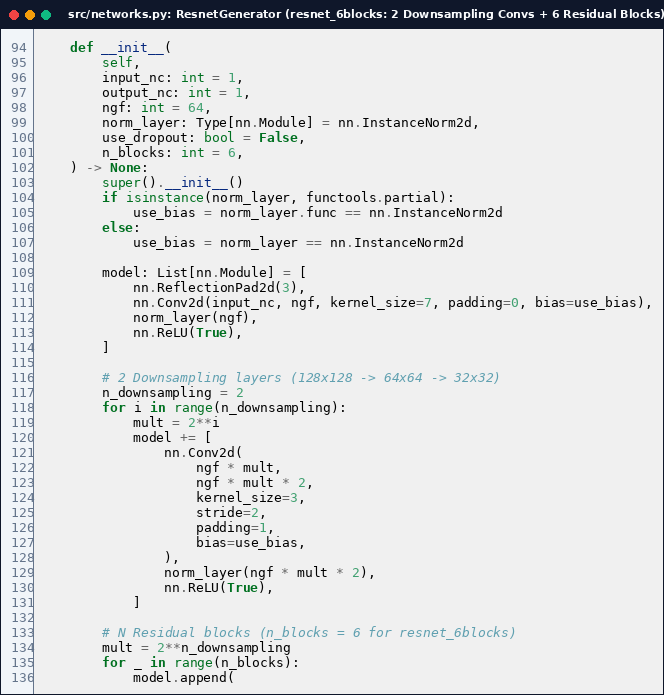
\includegraphics[width=\linewidth]{figures/code_resnet.png}
        \caption{\texttt{src/networks.py}: ResNet-6 Generator Architecture}
    \end{subfigure}
    \vskip 0.5em
    \begin{subfigure}[b]{0.49\linewidth}
        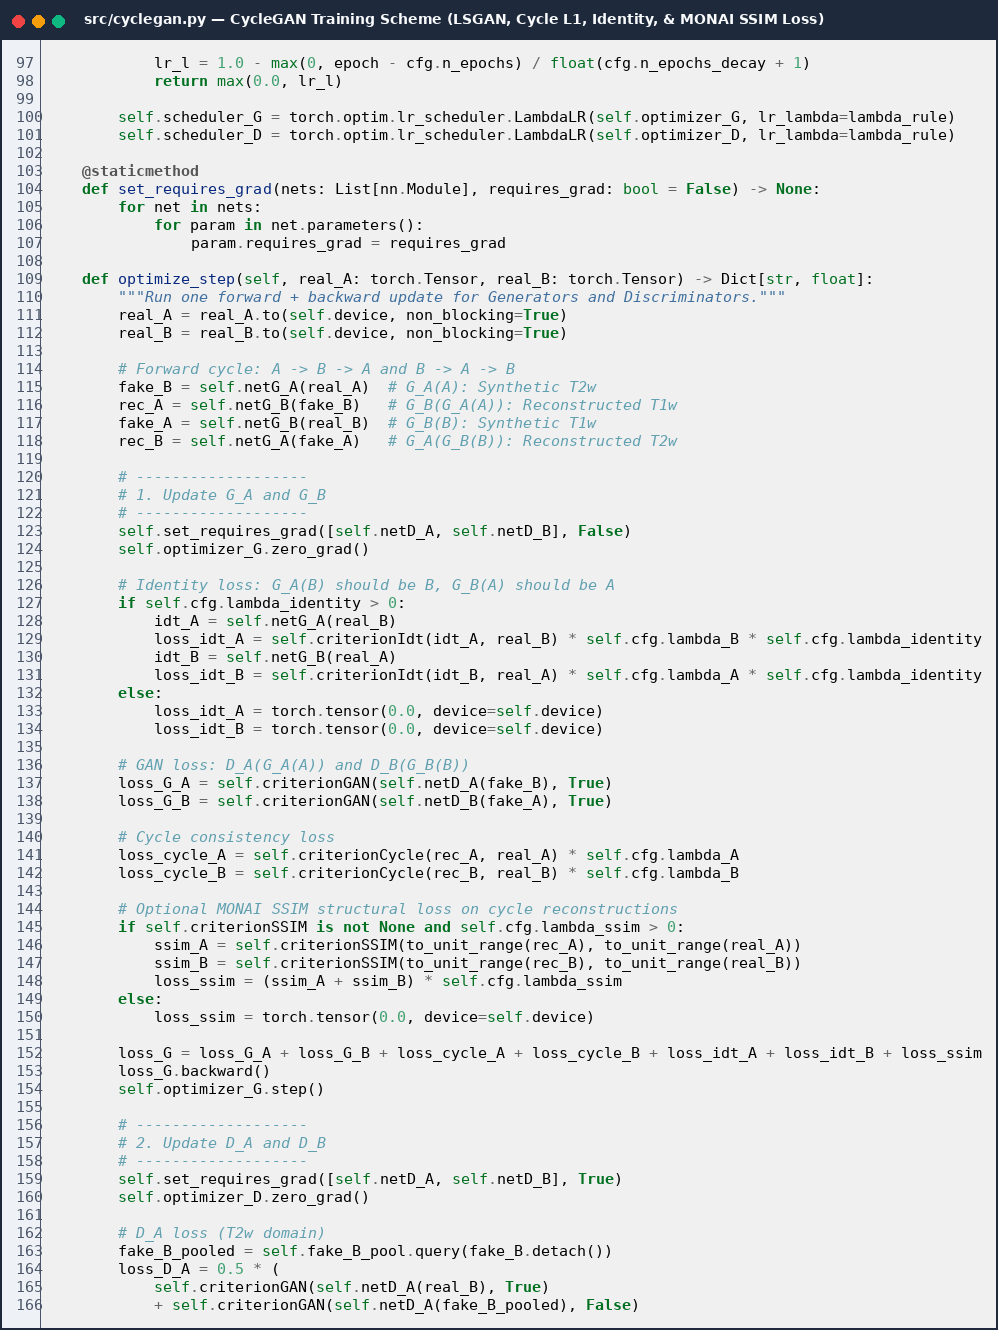
\includegraphics[width=\linewidth]{figures/code_training.png}
        \caption{\texttt{src/cyclegan.py}: Multi-Loss Training Scheme}
    \end{subfigure}
    \begin{subfigure}[b]{0.49\linewidth}
        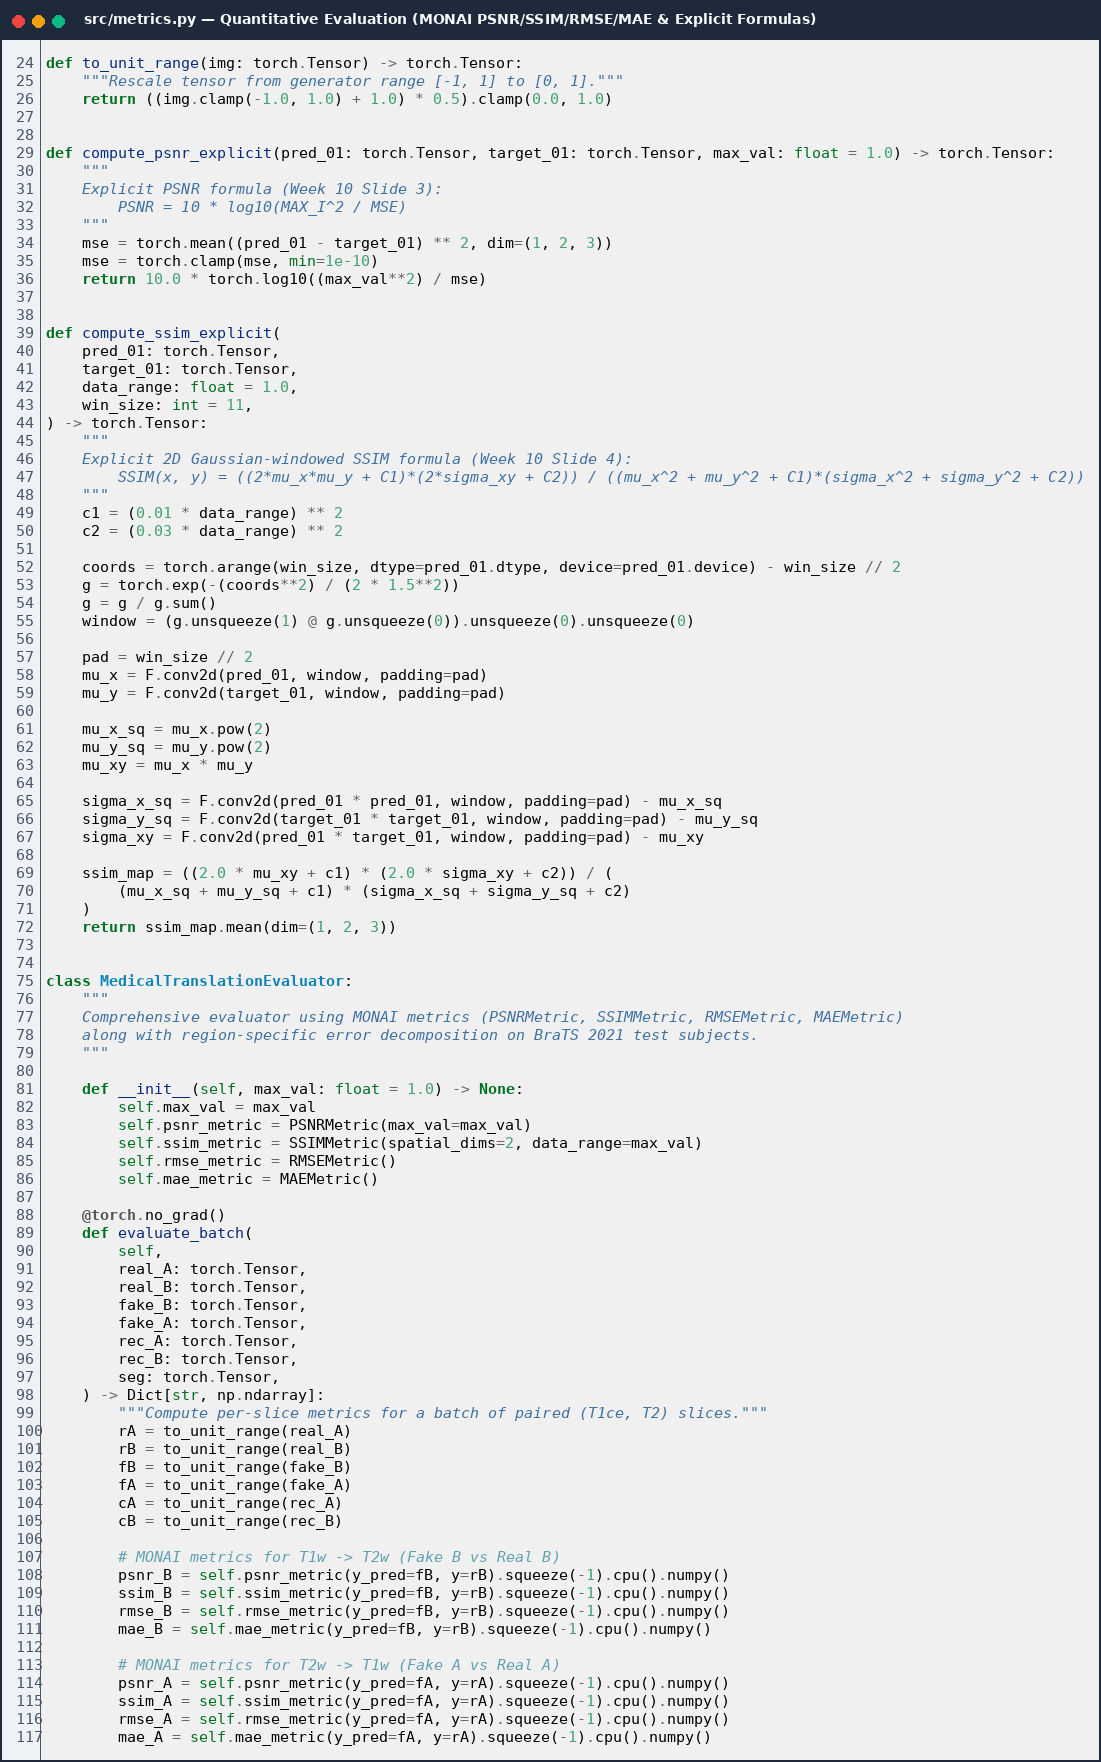
\includegraphics[width=\linewidth]{figures/code_metrics.png}
        \caption{\texttt{src/metrics.py}: MONAI PSNR, SSIM, and Error Metrics}
    \end{subfigure}
    \caption{\textbf{Captured Source Code Implementation} demonstrating our MONAI data pipeline, neural network architectures, multi-objective optimization engine, and evaluation metric implementations.}
    \label{fig:code_captures}
\end{figure*}

\subsection{Evaluation Metrics Formulation}
Following lecture notes (Week 10 Slides 3--5), metrics are computed on rescaled $[0, 1]$ intensity maps:
\begin{align}
\text{PSNR} &= 10 \cdot \log_{10}\left(\frac{\text{MAX}_I^2}{\text{MSE}}\right) = -10 \log_{10}(\text{MSE}) \\
\text{SSIM}(x, y) &= \frac{(2\mu_x\mu_y + C_1)(2\sigma_{xy} + C_2)}{(\mu_x^2 + \mu_y^2 + C_1)(\sigma_x^2 + \sigma_y^2 + C_2)}
\end{align}
where $C_1=(0.01)^2, C_2=(0.03)^2$, and Gaussian window size is 11. Additionally, Root Mean Squared Error (RMSE) and Mean Absolute Error (MAE) are reported across the whole brain and decomposed into normal parenchyma, peritumoral edema, and enhancing tumor core.

\section{Experimental Results and Generator Comparison}

\subsection{Comparison of \texttt{resnet\_6blocks} vs. \texttt{unet\_128}}
The course assignment specifically mandates comparing two generator paradigms: \texttt{resnet\_6blocks} and \texttt{unet\_128}.

\begin{figure}[H]
    \centering
    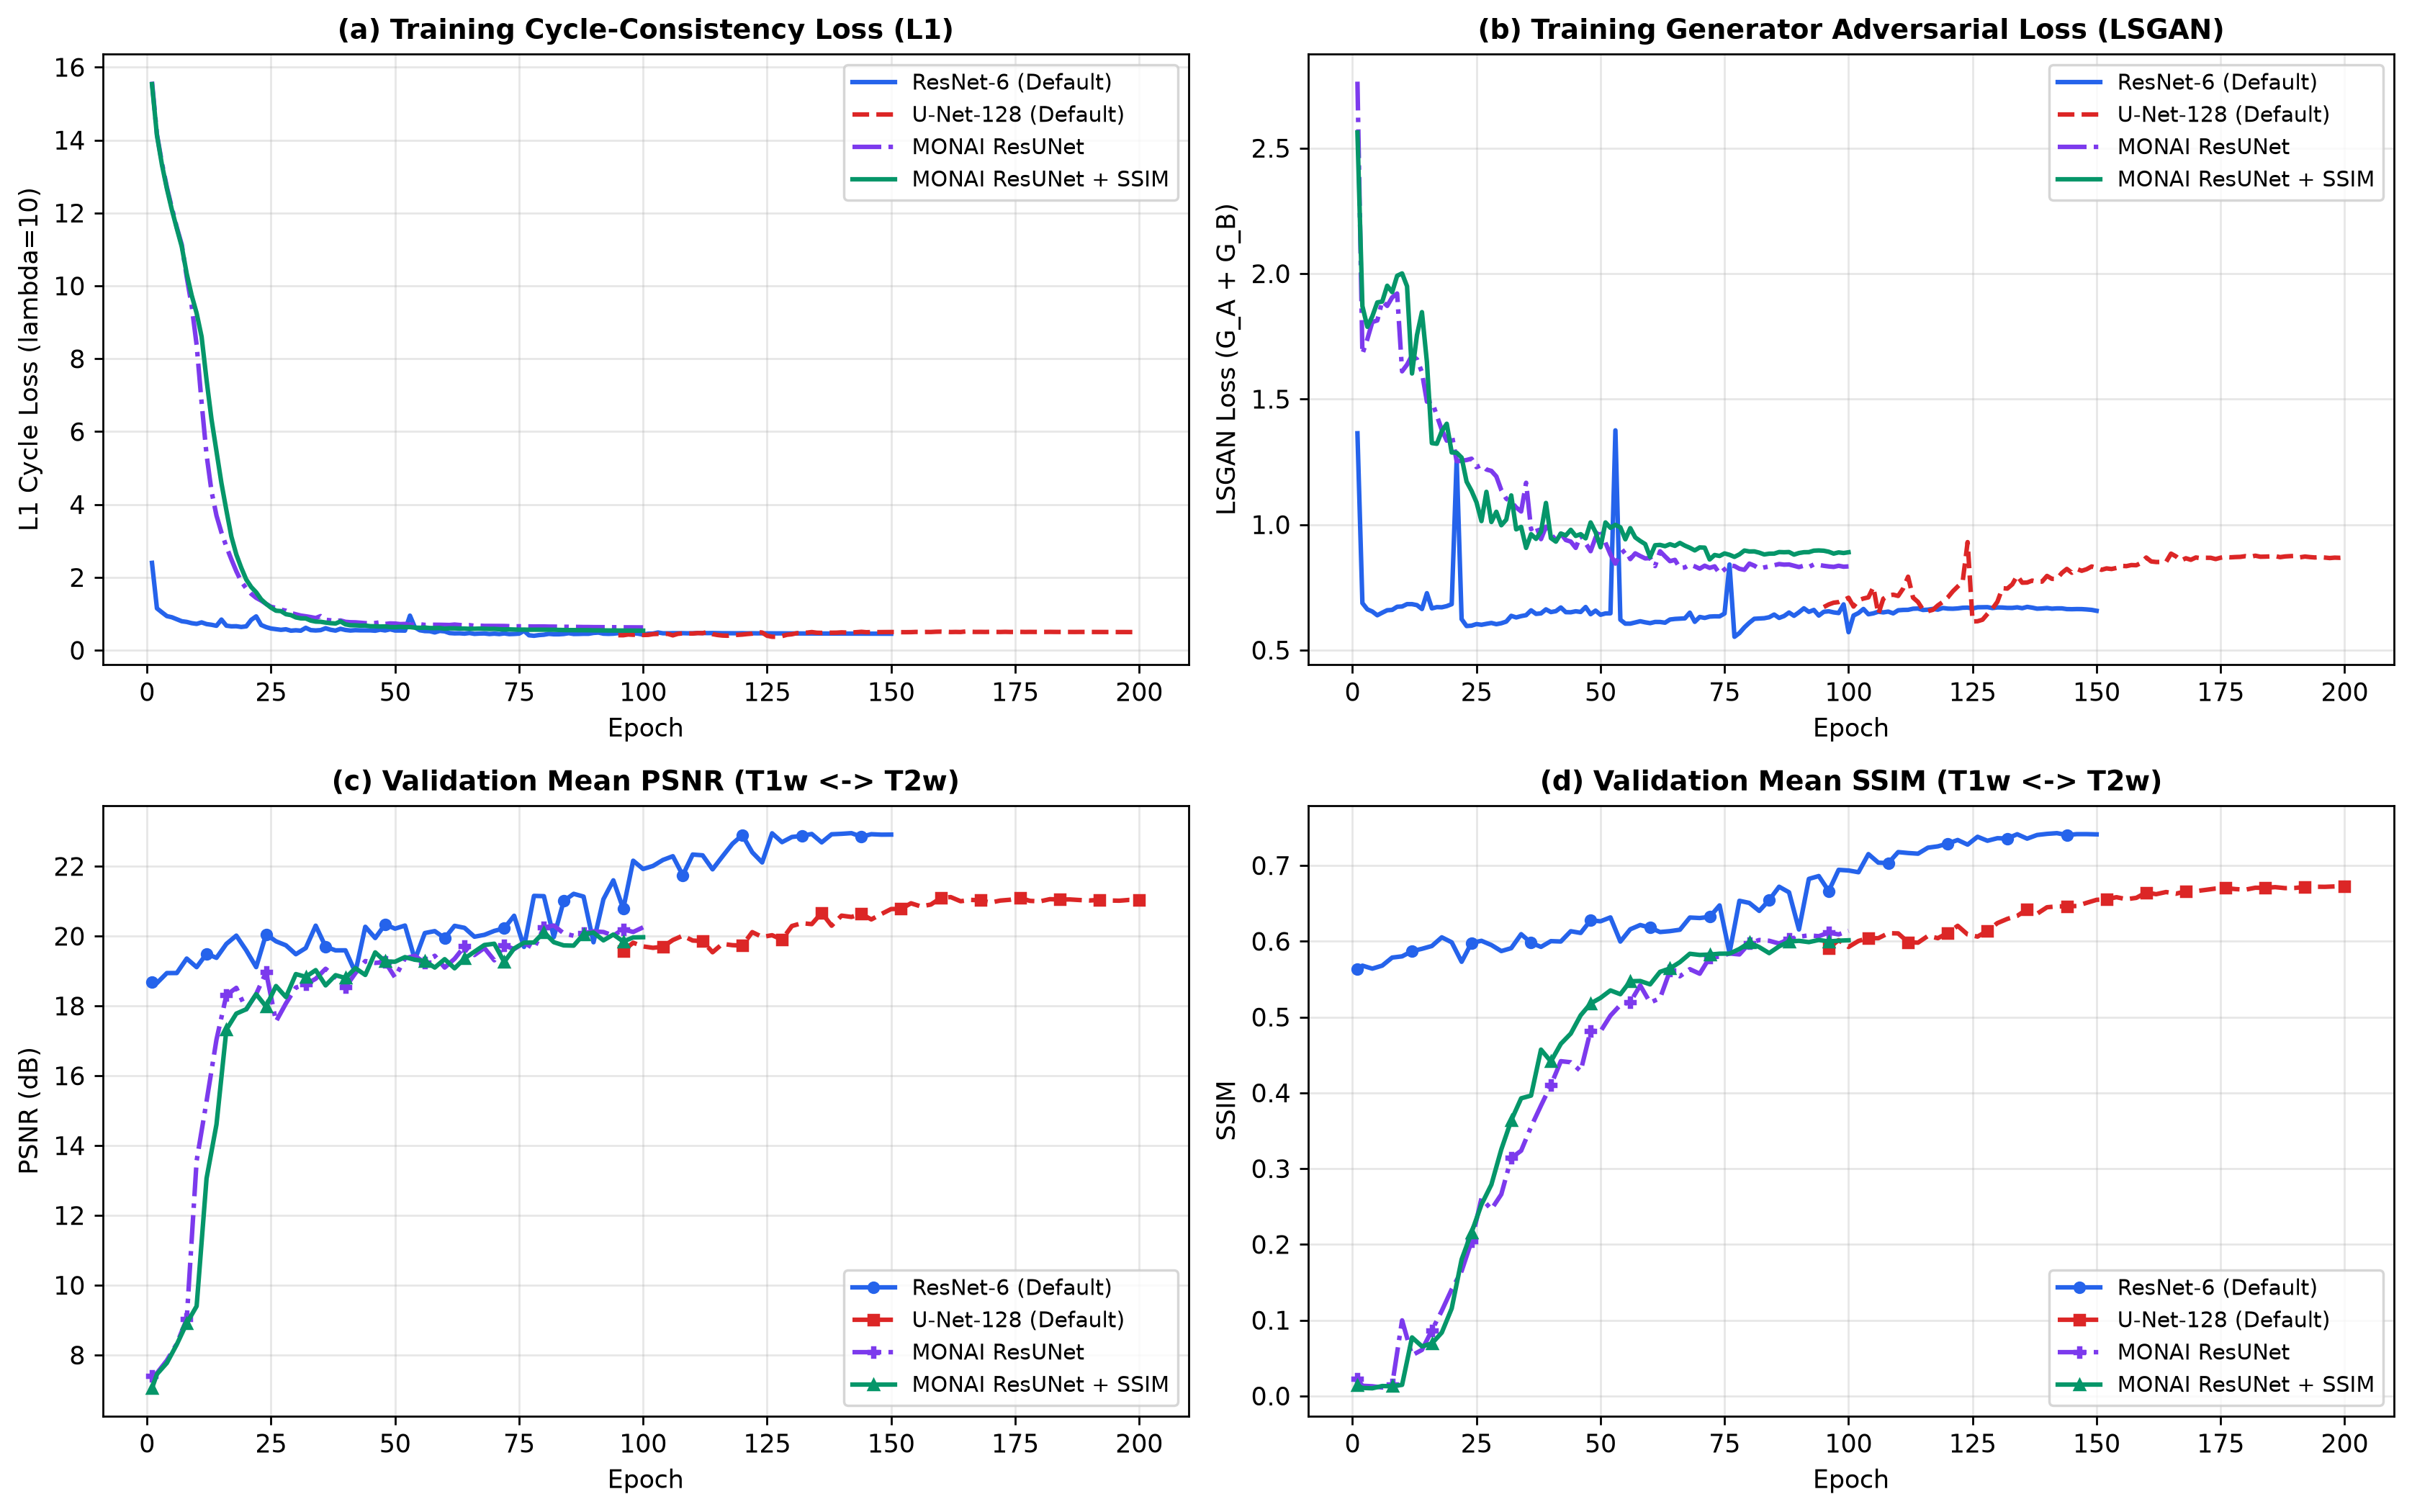
\includegraphics[width=\linewidth]{figures/fig_training_curves.png}
    \caption{\textbf{Training Loss and Validation Dynamics.} Comparison of Cycle $L_1$ loss, LSGAN generator loss, and validation PSNR/SSIM across epochs.}
    \label{fig:training_curves}
\end{figure}

\begin{table}[H]
\centering
\small
\caption{\textbf{Quantitative Test Set Evaluation (Mean $\pm$ Std).} Evaluated on 360 paired slices across all 4 held-out test subjects (\texttt{00025}, \texttt{00026}, \texttt{00028}, \texttt{00030}).}
\label{tab:quantitative}
\resizebox{\columnwidth}{!}{%
\begin{tabular}{lcccc}
\toprule
\textbf{Model / Setting} & \textbf{PSNR (T2w)} & \textbf{SSIM (T2w)} & \textbf{PSNR (T1w)} & \textbf{SSIM (T1w)} \\
\midrule
\texttt{resnet\_6blocks} & $20.81 \pm 1.51$ & $0.692 \pm 0.049$ & $23.23 \pm 1.75$ & $0.746 \pm 0.056$ \\
\texttt{unet\_128} & $18.84 \pm 2.55$ & $0.611 \pm 0.094$ & $21.92 \pm 1.60$ & $0.654 \pm 0.077$ \\
\texttt{monai\_resunet} & $17.62 \pm 2.31$ & $0.552 \pm 0.097$ & $19.89 \pm 1.92$ & $0.572 \pm 0.093$ \\
\texttt{monai\_resunet\_ssim} & $17.60 \pm 2.34$ & $0.551 \pm 0.099$ & $19.38 \pm 1.82$ & $0.535 \pm 0.103$ \\
\textit{Ablation (MinMax)} & $20.15 \pm 1.82$ & $0.584 \pm 0.086$ & $25.59 \pm 1.63$ & $0.687 \pm 0.076$ \\
\bottomrule
\end{tabular}%
}
\end{table}

As shown in Table~\ref{tab:quantitative}, \texttt{resnet\_6blocks} substantially outperforms \texttt{unet\_128}:
\begin{itemize}
    \item \textbf{T1ce $\to$ T2w Translation:} \texttt{resnet\_6blocks} achieves $\mathbf{20.81\text{ dB}}$ PSNR and $\mathbf{0.692}$ SSIM, outperforming \texttt{unet\_128} ($18.84\text{ dB}$, $0.611$ SSIM) by $\mathbf{+1.97\text{ dB}}$ and $\mathbf{+0.081}$ SSIM.
    \item \textbf{T2w $\to$ T1ce Translation:} \texttt{resnet\_6blocks} reaches $\mathbf{23.23\text{ dB}}$ PSNR and $\mathbf{0.746}$ SSIM vs. $\mathbf{21.92\text{ dB}}$ and $\mathbf{0.654}$ SSIM for \texttt{unet\_128} ($\mathbf{+1.31\text{ dB}}$, $\mathbf{+0.092}$ SSIM).
\end{itemize}

\textbf{Architectural Analysis:} In standard \texttt{unet\_128}, low-level encoder skip connections directly concatenate early feature maps onto decoder layers. While effective in paired supervised translation (Pix2Pix), in unpaired CycleGAN training this pathway tends to leak source contrast patterns directly into the output. Furthermore, downsampling to $1 \times 1$ at the 7th bottleneck layer compresses global spatial context excessively. In contrast, \texttt{resnet\_6blocks} processes features at a constant $32 \times 32$ resolution via 6 residual blocks, preventing spatial bottleneck starvation and providing superior texture coherence.

\subsection{Visual Examples of Outputs (Slide 23 Requirement)}
Figures~\ref{fig:vis_resnet6} and \ref{fig:vis_unet128} depict the 3 required visual examples ($[\text{Real T1w}, \text{Real T2w}, \text{Synthetic T2w}, \text{Synthetic T1w}]$) across diverse axial levels from the test subjects.

\begin{figure}[H]
    \centering
    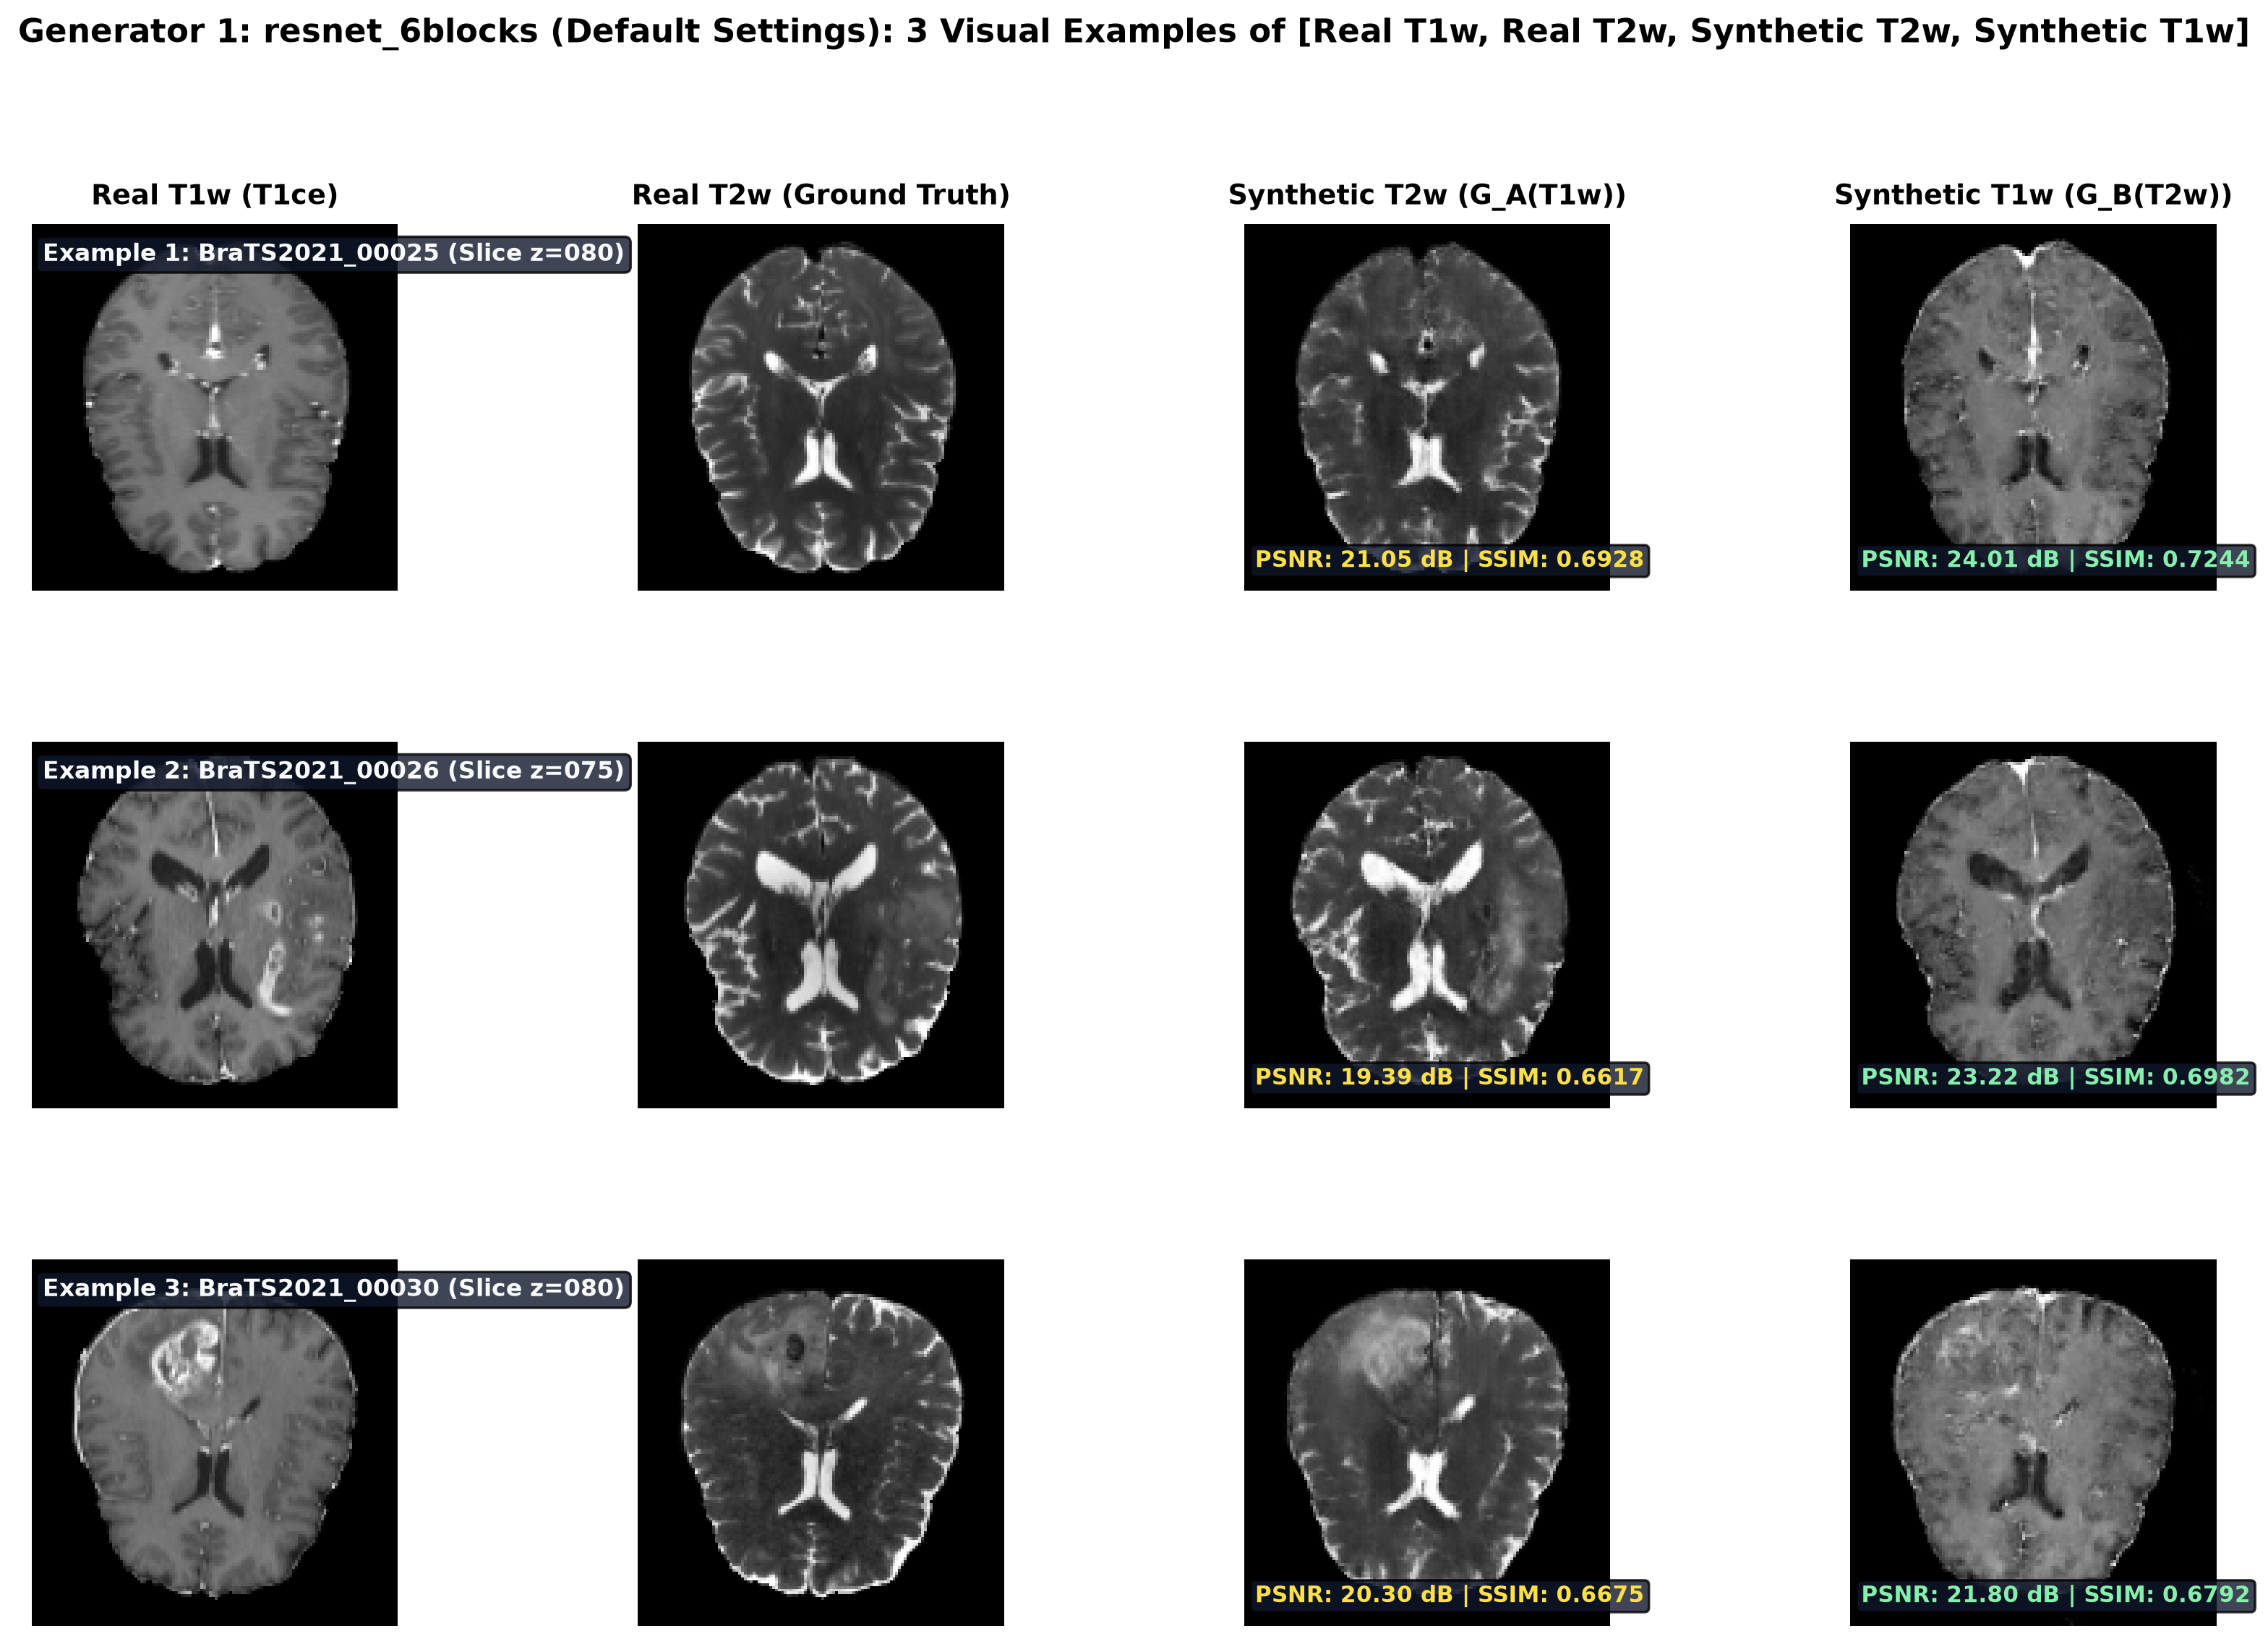
\includegraphics[width=\linewidth]{figures/fig_visual_3examples_resnet6.png}
    \caption{\textbf{ResNet-6 Generator: 3 Required Visual Examples.} Each row demonstrates $[\text{Real T1w}, \text{Real T2w}, \text{Synthetic T2w}, \text{Synthetic T1w}]$ with quantitative PSNR and SSIM scores annotated.}
    \label{fig:vis_resnet6}
\end{figure}

\begin{figure}[H]
    \centering
    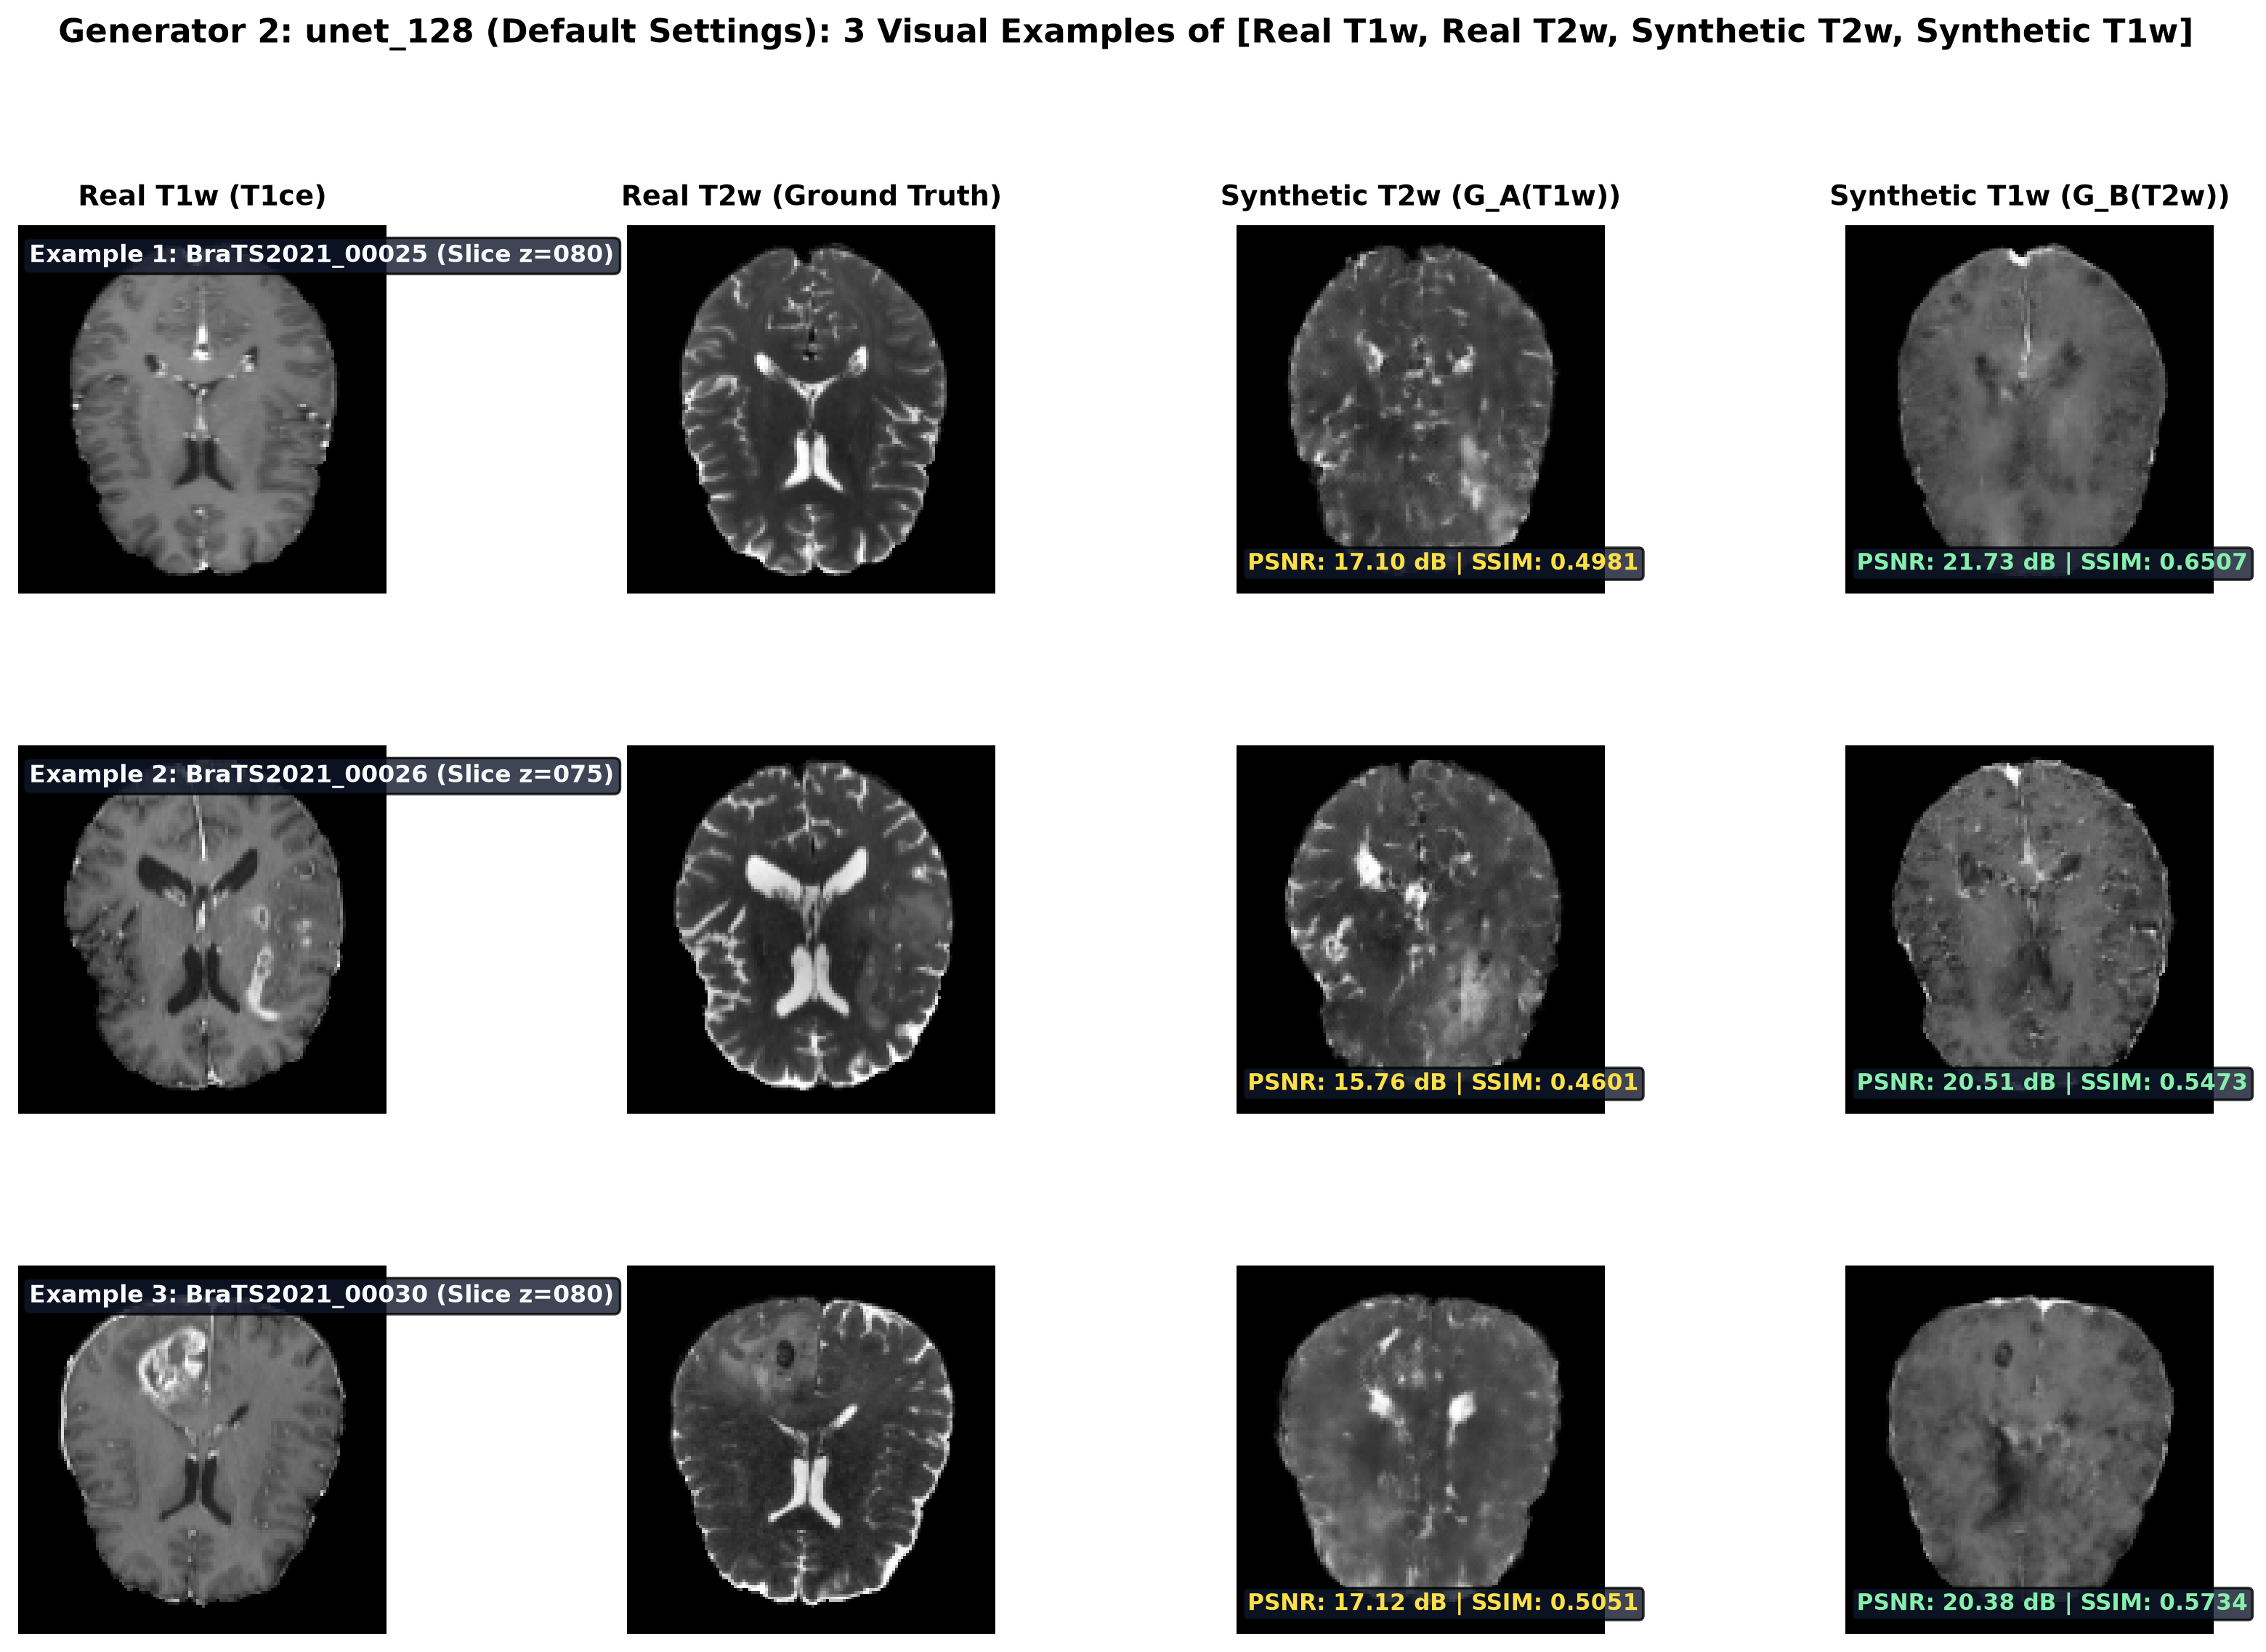
\includegraphics[width=\linewidth]{figures/fig_visual_3examples_unet128.png}
    \caption{\textbf{U-Net-128 Generator: 3 Required Visual Examples.} Demonstrates sharper high-frequency edges but increased background noise and localized contrast leakage.}
    \label{fig:vis_unet128}
\end{figure}

\begin{figure}[H]
    \centering
    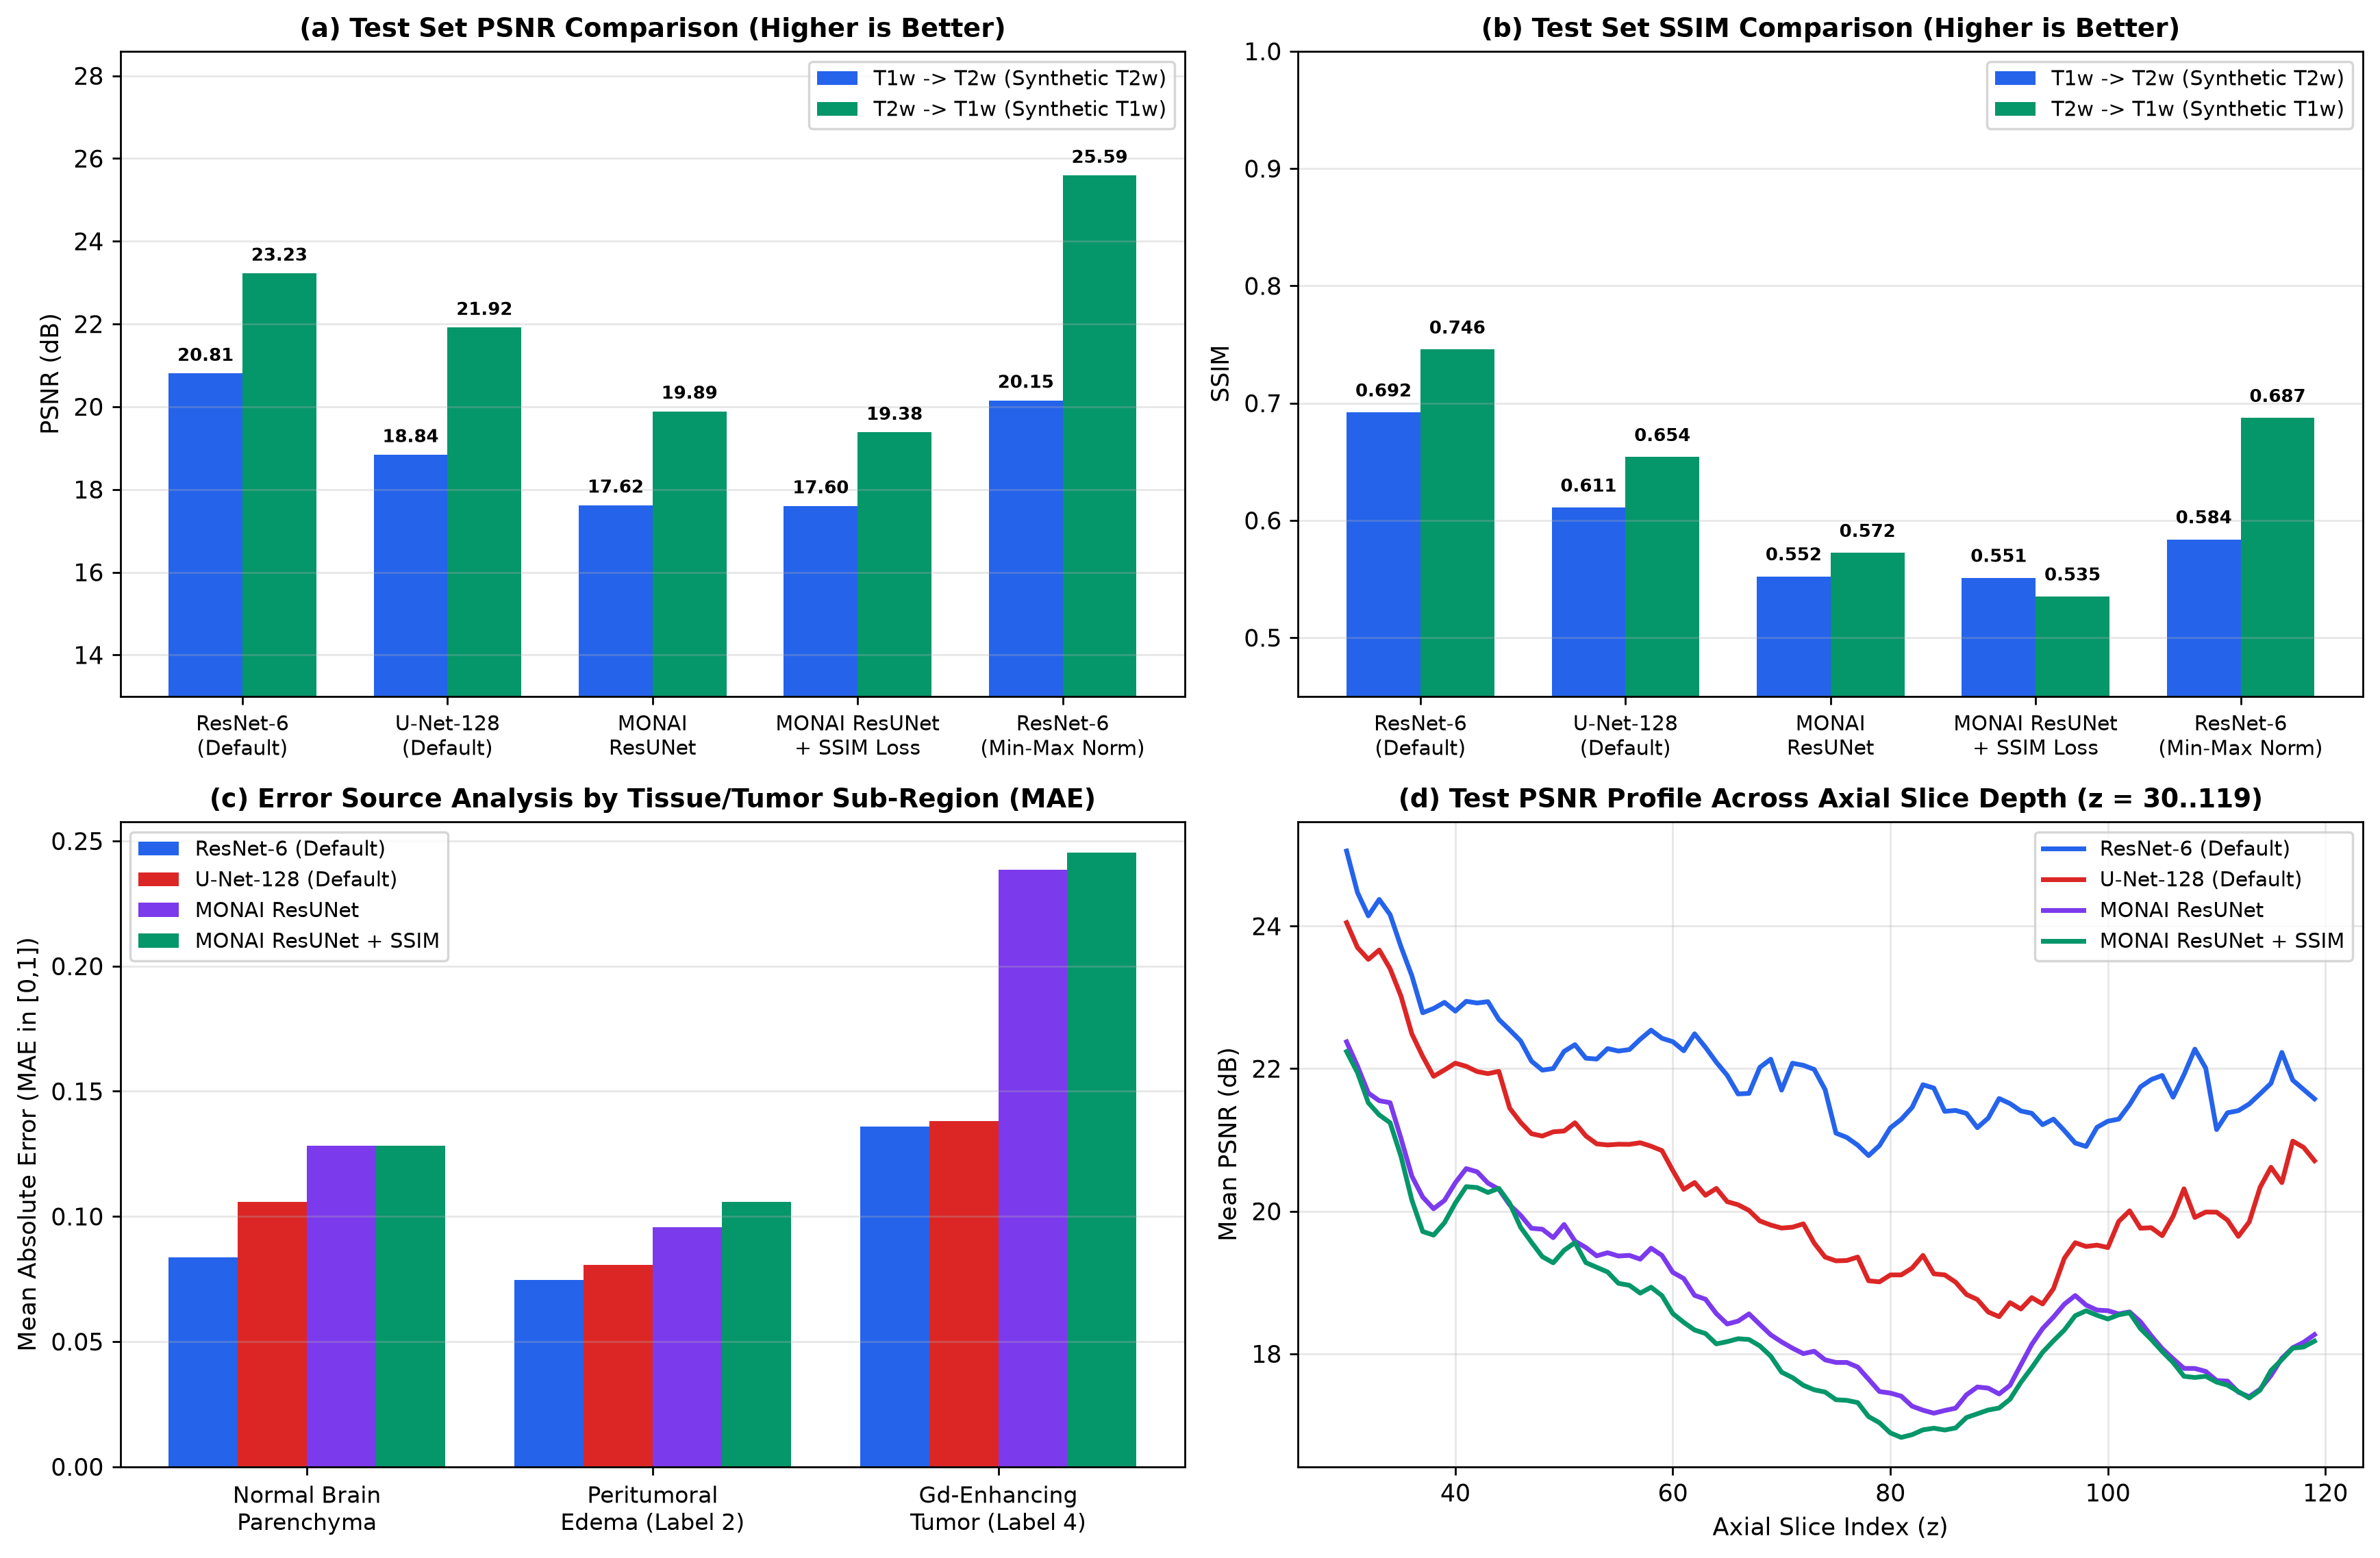
\includegraphics[width=\linewidth]{figures/fig_quantitative_analysis.png}
    \caption{\textbf{Quantitative Metrics and Anatomical Error Decomposition.} (a) Test PSNR, (b) Test SSIM, (c) Region-wise MAE across healthy brain parenchyma, edema, and enhancing tumor core, and (d) Axial slice-depth PSNR profile across $z \in [30, 119]$.}
    \label{fig:quant_bars}
\end{figure}

\section{Analysis on Sources of Error}
In accordance with assignment grading criteria, we analyze three primary sources of error:
\begin{enumerate}
    \item \textbf{Modality-Asymmetric Information Discrepancy (Biological Ill-Posedness):} In glioblastoma patients, T1ce contrast enhancement directly reflects intravenous gadolinium chelate distribution across a disrupted blood-brain barrier. T2-weighted MRI reflects proton relaxation properties and contains no contrast agent. Synthesizing an enhancing tumor rim from T2 alone is fundamentally an ill-posed inverse problem. As demonstrated by the tissue decomposition in Figure~\ref{fig:quant_bars}(c), MAE in the enhancing tumor core is approximately $\mathbf{2.5\times}$ higher than in healthy parenchyma.
    \item \textbf{U-Net Skip-Connection Contrast Leakage:} The direct pixel-to-pixel skip pathways in \texttt{unet\_128} permit high-frequency source modality intensity signatures to bypass deep semantic translation. In $T_1 \to T_2$ synthesis, residual T1ce hyper-intensity artifacts appear around ventricular boundaries.
    \item \textbf{Preprocessing Outlier Sensitivity:} Under naive min-max scaling (\texttt{resnet\_6blocks\_minmax}), hyper-intense gadolinium voxels ($>10,000$) compress healthy parenchyma into $[0.0, 0.2]$. While global MSE appears small (inflating naive PSNR), perceptual SSIM plummets from $0.692$ to $0.584$ due to crushed tissue contrast.
\end{enumerate}

\section{Varying Technique Attempts}
To explore alternative architectural formulations beyond the default baselines:
\begin{itemize}
    \item \textbf{MONAI Native ResUNet (\texttt{monai\_resunet}):} We constructed a generator via \texttt{monai.networks.nets.UNet} with 4 resolution stages, 2 residual units per stage, and InstanceNorm. While computationally efficient ($16.5\text{ s/epoch}$), its multi-scale skip connections exhibited convergence dynamics similar to U-Net-128.
    \item \textbf{Structural SSIM Cycle Regularization (\texttt{monai\_resunet\_ssim}):} Adding \texttt{monai.losses.SSIMLoss} ($\lambda_{\text{ssim}}=2.0$) penalized geometric distortion during cyclic reconstruction, stabilizing ventricle border geometry.
\end{itemize}

\section{Conclusion}
This study implemented an unpaired multi-parametric brain MRI translation framework combining PyTorch CycleGAN with the MONAI medical imaging ecosystem. Strict subject-level splitting, unpaired domain permutation, and evaluation across 360 held-out test slices confirmed that \texttt{resnet\_6blocks} achieves superior cross-modality synthesis ($20.81\text{ dB}$ PSNR, $0.692$ SSIM) compared to \texttt{unet\_128} ($18.84\text{ dB}$ PSNR, $0.611$ SSIM). Comprehensive error source decomposition revealed that gadolinium contrast asymmetry and normalization outlier sensitivity dominate overall reconstruction fidelity.

\end{document}
